\chapter{Personal Home Automation Language}\label{sec:PersonalHomeAutomationLanguage}
As described in Chapter~\ref{ch:ProblemAnalysis}, the aim of this project is to develop a new programming language for the Arduino hardware platform that is intuitive to use for the users described in Section~\ref{ProblemA:Users}.
\\\\
In this section we will discuss the language criteria as defined by Robert W. Sebesta and relate it to the demographic of PHAL, and through these criteria determine the features that PHAL should support. We will investigate different programming paradigms to relate to the subject \textit{Home Automation}, and compare the definition of PHAL to the current Arduino language. Finally, we will show some code examples written in PHAL to show the syntax of the language.

\section{Initial design of the PHAL language}
When designing a new programming language for the Arduino, the first step is to determine which features the programming language should implement. This is an essential part of the early development, since it lays the foundation for the rest of the development.  

\subsection{Syntactical brainstorm}
To come up with new ideas for a language, we had each of the designers perform a series of assignments to brainstorm the syntactical format of the language. They would imagine a new language that they thought to be fitting to the demographic and construct some code examples as shown on Listing~\ref{code:InitialExerciseCodeWriting}. 
\begin{lstlisting}[caption={This listing shows how a designer imagined the new language to look like}, label={code:InitialExerciseCodeWriting}]
TempSensor temp_indoor = 1
TempSensor temp_outdoor = 2
WindowController window = 3
Radiator rad = 4

if(temp_indoor.reading < 20)
  until(temp_indoor.reading > 20)
    rad.increase()

if(temp_indoor.reading > 30)
  if(temp_outdoor.reading > 10 & temp_outdoor.reading < 30)
    until(temp_indoor.reading < 25)
      rad.off()
      window.open()

window.close()
\end{lstlisting}
This forced the designers to be creative, and it helped to see what the other designers thought the new language could look like, and which features they wished to include. The different language syntaxes were discussed, serving to create a foundation for a language based on compromises. The compromise of this exercise would end up determining the syntax of PHAL. 

\section{Language criteria}
In this subsection we will examine the language criteria proposed by Robert W. Sebesta in the book Concepts of Programming Languages \cite{Sebesta}. These criteria are used for evaluation in accordance with the targeted problem domain. Figure \ref{fig:LanguageCriteria} shows the different criteria. 

\begin{figure}[H]
\centering
  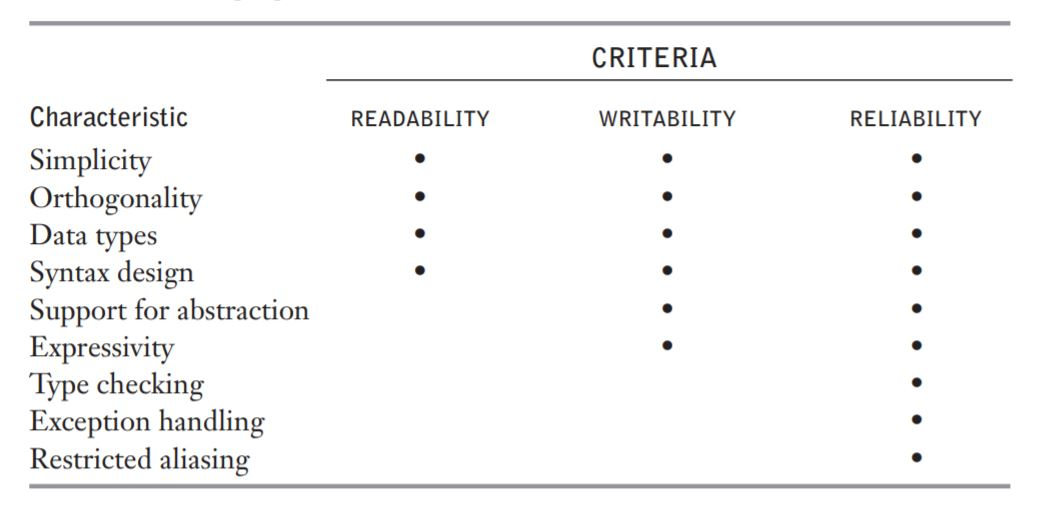
\includegraphics[scale=0.8]{figures/Analysis/sebestecriteria.JPG}
  \caption{This figure shows the language criteria proposed in Sebesta's book \cite{Sebesta}.}
  \label{fig:LanguageCriteria}
\end{figure}
\noindent
As shown, there are three major language criteria: readability, writability and reliability \cite{Sebesta}. The figure shows how the different characteristics affect them.
\begin{itemize}
    \item \textbf{Readability} pertains to the ease with which programs can be read and understood
    \item \textbf{Writability} is a measure of how easily a language can be used to create programs for a chosen problem domain
    \item \textbf{Reliability} relates to whether a program is able to perform to its specifications under all conditions
\end{itemize}
Since PHAL is targeted at users with limited programming experience as seen in Section \ref{ProblemA:Users}, and as such the language criteria valued the highest are the ones that we envision would help the demographic the most. These are simplicity, data types, syntax design, expressivity and type checking.

\subsection{Characteristics for language criteria}\label{subsec:CharacteristicsForLanguage}
In the following, the characteristics deemed relevant for PHAL will be described.

\subsubsection{Overall simplicity}
The overall simplicity of a language is tied to all of the main criteria, but strongly affects the readability of a language. This pertains to the amount of basic constructs contained in a language - more constructs mean it is harder to learn. This also relates to feature multiplicity, meaning multiple ways to accomplish the same goal should be avoided for simplicity. Operator overloading can also cause simplicity issues if used in excess of what is needed.
\\\\
This is especially relevant for PHAL. The language, as specified in Section~\ref{ProblemA:Users}, is targeted at hobbyists with a limited prior knowledge about programming. This means the language should aim to be as simple as possible for these programmers. PHAL should be comprised of few constructs, and these should be as easy to understand as possible to ensure simplicity. In accordance with the definition of simplicity, PHAL should include operator overloading where it makes sense while avoiding excessive use. The specific rules for overloading in PHAL will be discussed later in Section~\ref{subsec:FormalTypeRules}, where the type rules are discussed.

\subsubsection{Data types}
This relates to the ability to define data types and structures, and aids the readability of the program, for example through the use of \textit{true} and \textit{false} rather than $1$ and $0$.
\\\\
This is relevant for the same reasons as overall simplicity. PHAL needs to define data types that are as simple to use as possible, while giving the user the proper functionality required for home automation. The considerations made in regards to this, and the final types to be implemented are further discussed during the language definition in Chapter~\ref{ch:LanguageDefinitions}, and more in depth in the \textit{types} section, Section~\ref{Def:Types}.

\subsubsection{Syntax design}
This is the form of the elements of the language, which aids readability through use of intuitive keywords for the different tasks. 
\\
This is relevant for PHAL, as it is essential for all the major criteria. The language should be explicit in its syntax, and when performing operations an intuitive syntax should be ensured through relating the operations to general mathematical notation. The general syntax will be explained and used later in this report.

\subsubsection{Expressivity}
Expressivity means something can refer to several different characteristics. This relates to PHAL since the \textit{number} type is used for convenience rather than distinguishing between integers and floating point types.
On top of this, the language aims to be more expressive in its control structures, by adding keywords such as \textit{times} and \textit{until} in loops.

\subsubsection{Type checking}
The purpose of type checking is to test for type errors in a given program. Being able to identify these increases the reliability of the language. 
\\\\
\textit{Type checking} is highly valued for PHAL because of the demographic. It is expected that the programmers will make mistakes, and as such need to take appropriate action when it happens, and inform the programmer of what they did wrong in order to correct them.
\\
Type checking will be further described in technical terms in Chapter~\ref{ch:typechecking}.

\section{Programming paradigms}
In order to make a new programming language it is necessary to choose a programming paradigm for the language. 
A programming paradigm is a certain approach to computer programming based upon a set of principles and concepts, making each particular paradigm superior at certain kinds of problems.
\\
It is therefore important to discuss this subject and which of these paradigms should be used as a foundation for PHAL.
\\\\
Programming paradigms are also used to classify programming languages into certain categories based on their features. A programming language may feature more than one paradigm, such as C\#, which incorporates both the object oriented as well as the declarative paradigms. Below are some of the most common programming paradigms \cite{ProgrammingParadigmsKurtNormark}:
\begin{itemize}
    \item \textbf{The imperative paradigm} is based upon a \textit{first do this and next do this} approach. The order in which the commands are given is very important for the program to execute correctly. Commands can typically be assignments, input/output or procedure calls. This paradigm is rooted in the idea of the digital computer and how it functions. Some languages that represent this paradigm are C, Fortran, Algol and Pascal
    \cite{ProgrammingParadigmsDefinition}
    \cite{ProgrammingParadigmsKurtNormark}.
    
    \item \textbf{The functional paradigm} originates from a mathematical standpoint - the theory of functions. Kurt Nørmark describes the paradigm as: 
    \begin{quote}
        \dots it is considered by many to be a more clean version compared to the imperative paradigm because the imperative paradigm is based on the more complicated digital computer \cite{ProgrammingParadigmsKurtNormark}.
    \end{quote}
    In the functional paradigm, functions are first-class values which means they can be passed as arguments, modified, assigned to a variable and returned from a function. 
    Functions also work as the primary flow control, meaning that the functions decide how the program executes compared to other paradigms where an if-statement or other selective control structures implement this functionality. 
    This increases the written code's readability and maintainability since every single function is made to handle a specific problem and is not reliant on any external state. 
    The sequence in which the commands are given is also not important in this paradigm. 
    Some languages that use this paradigm are Lisp, Haskell, Erlang and F\# \cite{ProgrammingParadigmsDefinition} \cite{FunctionProgrammingVsImperativeProgramming}.
    
    \item \textbf{The declarative paradigm} is quite different from the other paradigms. 
    Instead of writing how to get what you want, you simply write what you want and it is then up to the compiler to figure out how to get it. 
    This paradigm is used extensively in query languages such as SQL and has also made its way into languages such as C\# with the addition of the LINQ library \cite{ProgrammingParadigmsDefinition} \cite{ProgrammingParadigmsForDummies}. 
    
    \item \textbf{The object-oriented paradigm} is based on the concept of \textit{objects} which may contain data and methods. 
    Some of the appealing aspects of the object oriented paradigm is the strong support for encapsulation and the very intuitive way of grouping together program aspects. 
    The objects are often made from classes, which act as a blueprint, where the objects are individual instances of its class. 
    A class can inherit from another class, this feature has multiple positive effects. 
    One of them is to reduce code duplication and it also enables message passing which reduces the amount of code needed to be written.
    Some of the languages that use this paradigm are C\#, Java and PHP \cite{ProgrammingParadigmsDefinition} \cite{ProgrammingParadigmsKurtNormark}.

    \item \textbf{The logic paradigm} is not a paradigm that is seen often in the more general areas of computation. 
    On the other hand, this paradigm works especially well when extracting knowledge from a given set of facts and relations. 
    This paradigm is rule based, but the rules do not need to be specified in a certain order. 
    It is simply up to the implementation to decide how these rules fit together to give the desired result. 
    This makes it a very proficient paradigm when working with artificial intelligence. 
    One of the most popular languages using the logic paradigm is Prolog \cite{Sebesta} \cite{ProgrammingParadigmsDefinition} \cite{ProgrammingParadigmsKurtNormark}.
    
    \item \textbf{The structured paradigm} is much like the imperative paradigm, but with a heavy emphasis on structures. 
    Structures are subroutines, conditions and loops and these are used to manage the control flow of the program, rather than using \textit{GOTO's} which were traditionally used very liberally \cite{ProgrammingParadigmsDefinition}.
\end{itemize}
When determining the proper paradigms to base PHAL around it is necessary to keep the targeted users in mind to choose an appropriate approach. 
As determined in Section~\ref{ProblemA:Users}, the language is aimed at users that want to do home automation on a hobby level, and is therefore required to be an introduction to programming and facilitate ease of use for new programmers.
\\\\ 
On top of this, the application of the language needs to be considered. 
PHAL is designed for home automation, and because of this, some approaches lend themselves better to this purpose. 
Some functionality of certain approaches could be considered redundant, especially in conjunction with the assumption that the users would write fairly simple programs. 
For this reason, the object-oriented, logic and functional paradigms are discarded. 
In our experience, it is preferable to have prior programming experience to fully grasp the concept of functions and classes which are core concepts in these paradigms. 
\\
Furthermore the logical paradigm does not seem to fit the problem domain which our programming language is supposed to cover. 
\\\\
As the target users are inexperienced, we feel that the most appropriate approach would be a mix of the imperative, structured and declarative paradigm. 
This allows the user to construct their program in an easy to comprehend manner using the imperative paradigm, while still using abstract yet easy to understand control structures as used in the structured paradigm. 
This also allows them to do more complex operations without having to write the code for it, using the declarative paradigm.

\section{The immediate goal of PHAL}\label{sec:phalvsarduino}
The main purpose of this project is to develop a more user friendly programming language for the Arduino hardware platform, as described in Chapter~\ref{ch:ProblemAnalysis}, compared to the default language provided for the Arduino. 
\\\\
One of the methods we plan on using to accomplish this is by adding a higher level of abstraction. This will make it easier for novice programmers to understand and use the PHAL language. 
This is done by combining some of the types from the Arduino Programming Language into types that are easier to work with for novice programmers, and introduce some new features such as \textit{groups}. 
In accordance with the intended demographic and avoiding the need for extensive programming knowledge, ending statements with the \textit{;} character seemed unnecessary and complicated. 
Instead we chose to use the separation of lines to end a statement, which means that every time the programmer creates a new line the previous statement is ended.
\\\\
\textbf{Numbers} in the Arduino language numbers are divided into multiple types. 
These are \textit{int}, \textit{byte}, \textit{double}, \textit{float}, \textit{long} and \textit{short}. 
For the intended users it is very hard to distinguish between the different types and know when to use them \cite{FiveCommonArduinoMistakes}. 
In PHAL all these types have been removed so the programmer does not need to decide on which type to use. 
Instead, a new type called \textit{number} will be introduced as the only type to handle numbers in PHAL. 
It is then up to the compiler to decide at compile time which underlying data type should be used instead.
\\\\
\textbf{Logical operators} in the Arduino language are implemented in a way that can be confusing for the intended users, such as for example the \textit{equal} operator being written as a double equal sign \textit{==}. 
This is easy to mistake by using a single equal sign, which specifies an assignment. 
For the intended user this is a very common mistake \cite{FiveCommonArduinoMistakes}. 
PHAL introduces a new operator - \textit{is}, which has the same functionality as the equal sign, and thus allows the user to use either of them.
\\
In the same way, the programmer will be able to interchangeably use words instead of mathematical operators for comparisons. 
The list of equivalent expressions can be seen on table~\ref{table:phaloperators}.
\begin{table}[H]
\centering
\caption{PHAL Operators} \label{LA:PhalOperators}
\label{table:phaloperators}
\begin{tabular}{|l|l|}
\hline
\textbf{Mathematical} & \textbf{Linguistic}        \\ \hline
=                   & is                               \\ \hline
!=                  & is not                           \\ \hline
\textgreater        & greater than       \\ \hline
\textless           & less than                      \\ \hline
\textgreater=        & greater than or equal to        \\ \hline
\textless=           & less than or equal to           \\ \hline
|                   & or                  \\ \hline
\&                 & and                 \\ \hline
!                    & not                 \\ \hline
\end{tabular}
\end{table}
\noindent
\textbf{Variable assignments} in the Arduino language are done using the single equal sign. 
To avoid ambiguity and ensure simplicity for the logical operators, the $=$ is replaced with the $:=$ operator in PHAL.
\\\\
\textbf{Strings} in the Arduino language are handled as \textit{char} arrays where the programmer needs to allocate the correct size of the array. 
The size cannot be changed afterwards. 
If the strings grow larger during the execution of the program a new \textit{char} array needs to be allocated by the programmer. 
This is a problem not only for the intended user, but also for programmers with prior experience \cite{FiveCommonArduinoMistakes}. 
PHAL will add a layer of abstraction to this issue. 
The programmer will have the ability to use a new type called \textit{text} that will be more like C\#, where the compiler will set the length of the \textit{char} array to make it easier for the programmer.
\\\\
\textbf{Structs} in Arduino language are used in the same way as structs in C, which the intended users have trouble with \cite{FiveCommonArduinoMistakes}. 
PHAL introduces a new datatype called \textit{group} which will attempt to make it easier for the programmer to group different data types together. 
It will also facilitate the ability to perform an action on all members of a group. 
\\\\
The considerations described and choices made in this section have all been based on the intention of making a language targeted at the intended users that Section~\ref{ProblemA:Users} defined, in an attempt to increase the simplicity of creating a home automation system for users using the Arduino platform.

\section{Examples of PHAL constructs}\label{ExamplesOfPHALConstructs}
To illustrate the considerations of PHAL's syntax, some coding examples for the different constructs will be established in the following section. 
The examples will consists of a listing showcasing the desired syntax, and a short explanation detailing the listing. 
In the following sections we will take a quick, informal view at the syntax for PHAL. 
\subsection{Comments}
\begin{lstlisting}[caption={Example of comments},label={code:comments}] 
# single-line comment
/* multi-line
comment */
\end{lstlisting}
For comments, a single-line comment will be preceded by a pound sign, this allows the user to enter comments in the code, that won't be handled by the compiler.
For multi-line comments, \textit{/*} will be used to indicate the start of a comment, and the reversed format \textit{*/} will be used to indicate the ending of that same comment. 

\subsection{Selective control structures}
The if statement serves as a structure that ensures that parts of the code are only executed when specific conditions are met.
\begin{lstlisting}[caption={Example of an \textit{If} statement},label={code:If-statement}]
if(<condition>) then {
  <statements and/or declarations>
}
else if(<condition>) then {
  <statement and/or declarations>
}
else then{
  <statement and/or declarations>
}
\end{lstlisting}
The \textit{if} statement is used to check if a specific condition is met. If this condition is met, the body inside the \{\} will be executed. Likewise, \textit{else if} is used to string multiple if conditions together. The following \textit{else if} condition will only be checked if the previous \textit{if condition} is not met. 
Finally, the \textit{else then} is used to execute code, but only if the previous \textit{if statement's} conditions are not met.
\\\\
The \textit{switch} statement serves as a simplistic alternative to the \textit{if-statement}. It allows the program to execute different statements, depending on the result of the expression. 
\begin{lstlisting}[caption={Example of a \textit{Switch} statement},label={code:Switch-statement}]
switch(<expression>) {
  case <n>:
    <statement and/or declarations>
  case <m>:
    <statement and/or declarations>
  default:
    <statement and/or declarations>
}
\end{lstlisting}
Unlike most programming languages, PHAL does not allow fall-through of switch cases. This means that the statement will automatically break whenever a case matches and finishes executing.
\\
The \textit{default} keyword works like the \textit{else} functionality of an \textit{if-statement}, and will only be executed if none of the previous conditions have been met.

\subsection{Loop}
For iterative control structures, it was decided to discard the usual \textit{for, while} and \textit{do while loops} and instead go with a more readable \textit{loop} structure. There will be different variations of the \textit{loop} structure, specifically \textit{loop x times} and \textit{loop until <condition>}. 
In the second version, \textit{increase by} and \textit{decrease by}, which can be seen on listing \ref{code:Loopstatement2}, are introduced to the syntax to help simplify the loops. 
Increase by and decrease by are optional parameters for the structure. \\
The following examples show the construction of loops:
\\
\begin{lstlisting}[caption={Example of a \textit{Loop} statement using until},label={code:Loopstatement1}]
loop until x > 100 {
  <statements>
}
\end{lstlisting}

\begin{lstlisting}[caption={Example of \textit{loop} statements using increase by and decrease by},label={code:Loopstatement2}]
loop until x > 100 increase x by 2 {
  <statements>
}

loop until x < 100 decrease x by 5 {
  <statements>
}
\end{lstlisting}

\begin{lstlisting}[caption={Example of a \textit{Loop} statement},label={code:Loopstatement3}]
loop x times {
  <statements>
}
\end{lstlisting}

\subsection{Methods}
Methods will be split into two separate listings, defining and calling. 
For defining methods, the keywords used are \textit{define, with} and \textit{returntype}. 
These keywords are introduced in an attempt to create context for the programmer. 
Defining a method will be done as shown on Listing~\ref{code:MethodDeclParam}:
\begin{lstlisting}[caption={Method declaration},label={code:MethodDeclParam}, escapeinside={(*}{*)}]
define <MethodName> with (<parameter1 type> <parameter1 name>, <parameter2 type> <parameter2 name>), (*\dots*)) returntype <returntype>{
  <content>
return <return value>
}
\end{lstlisting}
When defining a method that takes no parameters, a \textit{none} keyword is introduced:
\begin{lstlisting}[caption={Method declaration},label={code:MethodDeclNoParam}]
define <MethodName> with (none) returntype <returntype>{
  <content>
  return <return value>
}
\end{lstlisting}
When calling methods a \textit{call} keyword is used, and the \textit{with} keyword that was introduced for defining is still used. This would result in method calls looking similar to Listing~\ref{code:MethodCall1}:\\
\begin{lstlisting}[caption={Example of a \textit{method call} with parameters},label={code:MethodCall1}]
call <MethodName> with (<parameter1>, <parameter2>, <parameter3>)
\end{lstlisting}
When calling a method with no parameters, the \textit{none} keyword is used as seen on Listing~\ref{code:MethodCall2}.
\\
\begin{lstlisting}[caption={Example of a \textit{Method call} without parameters},label={code:MethodCall2}]
call <MethodName> with (none)
\end{lstlisting}

\subsubsection{The wait method}
PHAL will support some default methods to optimise the language for the problem domain and facilitate ease of use.\\
One of these will be the \textit{wait} method, which allows the user to make the Arduino wait for a given amount of seconds before continuing execution. An example of the syntax of the method can be seen on Listing~\ref{code:wait}\\ \begin{lstlisting}[caption={Example of the wait method},label={code:wait}]
wait 24.2 seconds
wait 2 seconds
\end{lstlisting}

\subsection{Including external libraries}
When using non-standard modules, eg. modules which are not natively supported by the language, external libraries can be included in the top of the file using the \textit{using} keyword followed by the library name as seen on Listing~\ref{code:includingLibrary}.  

\begin{lstlisting}[caption={Example of including an external library},label={code:includingLibrary}]
using <library name>
\end{lstlisting}

\section{Code examples}
On Listing~\ref{code:InitialSampleCode2} is an example of a program that has been created to demonstrate our thoughts for the language and how it could potentially look. 
Additional code examples can be found in Appendix~\ref{APP:examples}.

\begin{lstlisting}[caption={Sample code}, label={code:InitialSampleCode2}]
/*****************************************************
 * Program purpose:                                  *
 * The purpose of this program is to evaluate the    *
 * temperature within a room and increase the        *
 * temperature. If the temperature is too high, open *
 * a window using a motor.                           *
 *****************************************************/

setup {
  temperatureSensor tmp := pin 3, 2
  
  motor motorOpen := pin 5
  motor motorClose := pin 6
  
  number tmpLow := 19
  number tmpHigh := 26
}

repeat {
  if(tmp.reading greater than tmpHigh) {
    closeWindow(motorClose)
  } else if(tmp.reading less than tmpLow ) {
    openWindow(motorOpen)
  }
}

define openWindow with (motor open) returnType none {
  open := true
  wait 3 seconds
  open := false
}

define closeWindow with (motor close) returnType none {
  close := on
  wait 3 seconds
  close := off
}
\end{lstlisting}
Listing~\ref{code:InitialSampleCode2} shows the use of a temperature sensor and motor component. 
The temperature sensor is used to measure the temperature in a room. 
The temperature can be accessed by using the .reading modifier on the components as seen on line 22 and 14. 
The wait function is used to pause the program for an specified amount of seconds. 
In this listing it is used to ensure that the motors are turned of again after they have been running for 3 seconds. 

\section{MosCoW}\label{section:moscow}
To limit the scope of the project, the MosCoW method has been applied to keep the focus on the important matters of the project. 
The MosCoW method describes which aspects of the work is deemed a must for the project to be successful. 
Furthermore, it describes what the project should have but is not a main priority. 
Then, it describes what the project could have if time allows, and finally it describes what is deemed irrelevant for the project at this time, but that could be implemented later on were the project to continue. 
\\\\
The MosCoW for the project is as follows:
\\\\
\noindent\textbf{Must have:}
\begin{itemize}
    \item Setup - Repeat format
    \item Variables and control structures
    \item Ability to define and use functions
    \item Functional types:
    \begin{itemize}
        \item Number
        \begin{itemize}
            \item Has the ability to be a integer or a decimal number
        \end{itemize}
        \item Bool
        \begin{itemize}
            \item Have values of either true or false
            \item Use of the on and off aliases for true and false
        \end{itemize}
        \item Text
        \begin{itemize}
            \item Contains a sequence of characters
            \item Needs the ability to concatenate texts together with the $+$ operator
        \end{itemize}
        \item Component
        \begin{itemize}
            \item Ability to turn component types on and off
            \item Assigning pins to components without having to specify if it is an output or input pin
        \end{itemize}
    \end{itemize}
    \item Group type that groups components together
        \begin{itemize}
            \item Ability to apply a single operation to all members of the group
        \end{itemize}
    \item Lists
        \begin{itemize}
            \item Ability to group variables of the same type together
            \item Must be able to iterate through the content of a list
        \end{itemize}
    \item Support of light or LEDs
    \item Selective control structures
\end{itemize}

\noindent\textbf{Should have:}
\begin{itemize}
    \item Linguistic logical statements
    \item Ability to perform operations on groups
    \item Ability to read sensor components
    \item Iterative control structures
\end{itemize}

\noindent\textbf{Could have:}
\begin{itemize}
    \item Support of heating systems
    \item Support of motion sensors
    \item Ability to include libraries
    \item Some pre-programmed component libraries
    \item A reference keyword that allows parameters to be passed as a reference instead of value 
\end{itemize}

\noindent\textbf{Won't have (at this time):}
\begin{itemize}
    \item A complete library of components used in Arduino
    \item Ability to perform more complex operations on components that are specific to that component
\end{itemize}
\noindent
By including the points from the \textit{must have} part, a user will be able to write a minimalistic program that can control the light of the house, based on criteria controlled by a selective control structure.\\
With the \textit{should have} points, the user will be able to use additional hardware components, have further control of groups and the language will be expanded to reach a broader demographic unfamiliar with programming languages as defined in Section~\ref{ProblemA:Users}. These points were not deemed essential, but should be included in order for the language to be useful in a real-world context.\\
The \textit{could have} and \textit{won't have} points will further expand the amount of components that the user can use, by allowing the inclusion of external libraries and include further pre-programmed components. These are not necessary for the overall functionality of PHAL in regards to home automation, but are an obvious boon for the users if implemented.

\section{Summary}
With the goals and visions of PHAL in place, it is now possible to formally describe the language and the functionality hereof.
In the next chapter we will take a look at defining the syntax.